\documentclass{article}

% if you need to pass options to natbib, use, e.g.:
% \PassOptionsToPackage{numbers, compress}{natbib}
% before loading nips_2018

% ready for submission
\usepackage{nips_2018}

% to compile a preprint version, e.g., for submission to arXiv, add
% add the [preprint] option:
% \usepackage[preprint]{nips_2018}

% to compile a camera-ready version, add the [final] option, e.g.:
% \usepackage[final]{nips_2018}

% to avoid loading the natbib package, add option nonatbib:
% \usepackage[nonatbib]{nips_2018}

\usepackage[utf8]{inputenc} % allow utf-8 input
\usepackage[T1]{fontenc}    % use 8-bit T1 fonts
\usepackage{hyperref}       % hyperlinks
\usepackage{url}            % simple URL typesetting
\usepackage{booktabs}       % professional-quality tables
\usepackage{amsfonts}       % blackboard math symbols
\usepackage{nicefrac}       % compact symbols for 1/2, etc.
\usepackage{microtype}      % microtypography
\usepackage{graphicx}
\usepackage{caption}
\usepackage{subcaption}
\graphicspath{{./img/}}

\title{Iterated Communication Through Negotation}

% The \author macro works with any number of authors. There are two
% commands used to separate the names and addresses of multiple
% authors: \And and \AND.
%
% Using \And between authors leaves it to LaTeX to determine where to
% break the lines. Using \AND forces a line break at that point. So,
% if LaTeX puts 3 of 4 authors names on the first line, and the last
% on the second line, try using \AND instead of \And before the third
% author name.

\author{
  Michael~Noukhovitch\\
  MILA\\
  \texttt{michael.noukhovitch@umontreal.ca} \\
  %% examples of more authors
  %% \And
  %% Coauthor \\
  %% Affiliation \\
  %% Address \\
  %% \texttt{email} \\
  %% \AND
  %% Coauthor \\
  %% Affiliation \\
  %% Address \\
  %% \texttt{email} \\
  %% \And
  %% Coauthor \\
  %% Affiliation \\
  %% Address \\
  %% \texttt{email} \\
  %% \And
  %% Coauthor \\
  %% Affiliation \\
  %% Address \\
  %% \texttt{email} \\
}

\begin{document}

\maketitle

\begin{abstract}
  The abstract paragraph should be indented \nicefrac{1}{2}~inch
  (3~picas) on both the left- and right-hand margins. Use 10~point
  type, with a vertical spacing (leading) of 11~points.  The word
  \textbf{Abstract} must be centered, bold, and in point size 12. Two
  line spaces precede the abstract. The abstract must be limited to
  one paragraph.
\end{abstract}

\section{Introduction}

One of the first philosophers of language, Ludvig Wittgenstein, posited that
"language is use" \cite{wittgenstein2009philosophical}. This idea, that the use
of language is what gives it its meaning, is a profound statement that also has
consequences for how we think of language. Wittgenstein saw language as wholly
tied to its use, there could be no language separate from reality or possible
use. To this end, he defined language games as games with simpler forms of
language "consisting of language and the actions into which it is woven".

Recently, the AI community has taken this philosophy of language and sought to
use it as the basis for the communication of autonomous agents
\cite{wagner2003progress}. The field of "emergent communication" seeks to
understand language starting from the most basic of language games; the goal is
to teach agents to communicate amongst themselves grounded in a simpler world
described by some "game." This game can be one of

\section{Related Work}%
\label{sec:related_work}

\section{Reproduction and Criticism}%
\label{sec:reproduction}

\subsection{Reproduction}%
\label{sub:reproduction}
The reproduction code is an extension of Hugh Perkins' attempt at reproducing
the paper \url{https://github.com/ASAPPinc/emergent_comms_negotiation} with
many notable fixes and extensions. The paper itself is relatively reproducible
with strong prosocial agent results especially along the linguistic channel
and weaker non-linguistic

\subsection{Criticism}%
\label{sub:criticism}

Though the paper is quite good, there are still questions and issues that can be
raised.

\subsection{Prosocial Agents Don't Negotiate}%
\label{sub:prosocial_agents_don_t_negotiate}
A negotiation game where the interests of two parties do not clash is not as
much about negotiation as it is just sharing preferences and calculating the
optimum. This is exactly what is seen in case of prosocial agents with only a
linguistic channel: one agent communicates their preferences and the other
agent finds the optimal division and proposes it. In this way, the goal and even
the whole task is completely different for prosocial agents compared to selfish
agents whose selfish opponents do not have their best interests in mind. In this
way, selfish agents have no incentive to communicate their preferences as it
could potentially weaken their negotiating ability. In this way, we see that it
is not selfish agents failing to learn to communicate but learning to not
communicate not because they are selfish but because the situation does not
incentivise them to in a one-shot environment.


\subsection{Unmotivated Agents}%
\label{sub:unmotivated_agents}
The paper and unfinished repository both allow for sampling situations that give
no possible reward to an agent, either through sampling a pool with 0 objects of
any kind or sampling a utility for an agent such that there are no object for
which they have non-zero utility (e.g. [1,0,1]). In this case, any agent will
theoretically accept any opponent's offer but their reward will be $\frac{0}{0}$
and so pose an issue for calculating the fraction of possible reward which the
paper uses as a metric.

\subsection{Fractional Reward is Biased}%
\label{sub:fractional_reward_is_biased}
The metric used by the paper "fraction of joint reward" compares the reward
achieved by each agent (utility over the accepted proposal $u_i \cdot P$) with
the total reward possible. In the case of prosocial
agents the metric measures the optimality as both agents' rewards are the same (
an equally weighted sum of their individual rewards) and they seek to optimize
the total possible reward.

\begin{equation}
    FR_{\text{prosocial}} = \frac{u_A \cdot P + u_B \cdot P}{\max_P u_A \cdot P + u_B \cdot P}
\end{equation}

But in the case of selfish agents, the total possible reward is the not the
objective the agent is optimizing. The agents optimize their own reward and
using the total possible reward metric is therefore a bad way of judging
performance. Instead, you could measure how well each agent does at maximizing
their own reward, average across agents, and divide by the total possible reward

\begin{equation}
    FR_{\text{selfish}} = 0.5 * \frac{u_A \cdot P}{\max_P u_A \cdot P} + 0.5 * \frac{u_B \cdot P}{\max_P u_B \cdot P}
\end{equation}

But this is also wrong because the maximum possible reward for one agent will
usually decrease the reward for the opponent. In this way, the only situation where
$FR_{\text{selfish}} = 1$ is possible is if there do not exist any items for
which both agents have a non-zero utility. Since this situation is quite rare
(the whole point of negotiation is to resolve conflicting preferences) this
metric is unfair to selfish agents by usually being lower than for prosocial
agents and artificially makes them appear worse. Total possible reward is
therefore a bad metric for selfish agents and it is not conclusive that their
performance is worse.


\section{Exploratory Extensions}%
\label{sec:exploratory_experiments}

\subsection{Utility Channel}%
\label{sub:preferences_channel}
One way to test whether selfish agents are learning to communicate or whether
they are specifically learning not to communicate is to simulate what
information an agent could possibly communicate. Since the prosocial agents
learn to communicate their hidden utilites, it seems fitting to test if giving
full information of hidden utilities helps achieve better
results. To this end, we experiment with giving an agent information about the
opponent's utility similar to a communication channel. For selfish agents we
find that an agent tends to dominate its opponent if it knows the opponent's
preferences, and outcomes are relatively similar if neither agent knows the
opponent's preferences

\begin{figure}[h]
    \centering
    \begin{subfigure}{.5\textwidth}
    \begin{center}
        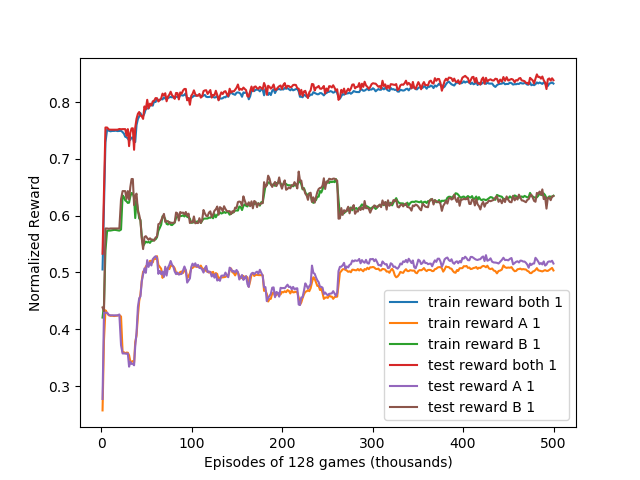
\includegraphics[width=0.9\linewidth]{opp-util-0.png}
    \end{center}
    \caption{agent B knows A's utilities}
    \end{subfigure}%
    \begin{subfigure}{.5\textwidth}
    \begin{center}
        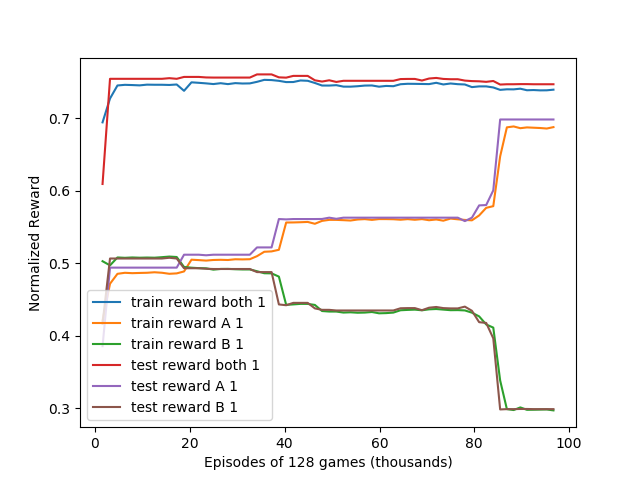
\includegraphics[width=0.9\linewidth]{opp-util-1.png}
    \end{center}
    \caption{agent A knows B's utilities}
    \end{subfigure}
    \label{fig:self-opp-util}
    \caption{The agent that knows the other's utilities, dominates}
\end{figure}

\subsection{Equitable Reward Metric}%
\label{sub:equitable_reward_metric}
Since fractional reward is biased as explained in
\ref{sub:fractional_reward_is_biased}, a better metric for selfish agents is
proposed to measure the performance of their negotiation: equitable reward.
Since each agent's preferences may be at odds with the other, it is better to
measure the agents' performances taking into account a comparison of their
respective utilities. We consider optimality if each agent recieves a proportion
of the items in the pool corresponding to the fraction of their utility over
their utility and their opponents. Essentially, if each agent recieves items
according to how much they care about them.

\begin{equation}
    ER_{\text{selfish}} = \frac{u_A \cdot P}{\frac{u_A}{u_A + u_B} \cdot P}
\end{equation}

Since for any given $P$ for selfish agents, $ER(A) = 1 - ER(B)$, we want to just
measure the optimality


\subsection{Utility Sampling}%
\label{sub:utility_sampling}
One consequence of randomly sampling utilities is that there is no
guarantee on the clash of utilities in negotation as the players could have
non-zero utility only for the items that their opponent has zero utility and
negotiation is simplified. To combat this issue, it is proposed to guaranteee
non-zero utility to every item.

Another issue is that in the social case, one player's utilities could dominate
the other's $u_j^1 > u_j^2 \forall j$. In such a case, the optimal strategy for
both players is to give all items to the player with the dominating utility, and
again the player. The final split is therefore pareto optimal, but doesn't feel
"fair" for the side of the dominated player. A similar situation for a selfish
agent would generally lead to a more even split with a smaller total reward. For
this reason, we can experiment with avoiding domination situations by
normalizing the utilities so that each agents utilities all sum to 15.

\section{Iterative Negotation}%
\label{sec:iterative_negotation}

\subsection{Pareto Optimality}%
\label{sub:pareto_optimality}

\section{Conclusion}%
\label{sec:conclusion}

\subsubsection*{Acknowledgments}

Use unnumbered third level headings for the acknowledgments. All
acknowledgments go at the end of the paper. Do not include
acknowledgments in the anonymized submission, only in the final paper.

\section*{References}

\bibliography{report}
\bibliographystyle{plain}

\end{document}
